\subsection{Previous work and usual approaches}
\label{section:registration_previous_work}
Several methods exist to estimate the transformation matrix. Iterative closest point (ICP) and other registration methods need an approximate initial guess to avoid converging in wrong local minima. They are applied directly in the 3D space. Other methods compute the 3D pose estimation of an object relative to the first and to the second camera from 2D images. Then they compute a transformation matrix to go from one view into the other one. This section develops some of the relevant approaches found in the literature.

% Other methods use 2D images. The strategy consists in:

% \begin{enumerate}
%     \item Finding keypoints/objects in the two images
%     \item Matching corresponding keypoints/objects in the two images
%     \item Finding
% \end{enumerate}

\subsubsection{Iterative closest point registration}
\label{section:Iterative closest point registration}

The ICP algorithm proposed by \cite{besl_method_1992} and \cite{chen_object_1992} is commonly used for alignment of 3D objects or scenes when an initial estimate of the relative pose is known. This algorithm is applied directly in the 3D space after the creation of the point clouds acquired from different views. The goal of ICP is to minimise the distance between two point sets.

$\mathbf{P}=\left\{p_{1} \ldots p_{N_{P}}\right\}$ is the target point cloud and $\mathbf{Q}=\left\{q_{1} \ldots q_{N_{Q}}\right\}$ is called the source point cloud.
 
 Different variants of ICP exist but they all iterate over the following steps in general:

\begin{enumerate}
    \item Select a subset of data from the two point clouds, $\mathbf{P}^{\prime}$ and $\mathbf{Q}^{\prime}$
    \item Find correspondences set $\mathcal{K} = \{(\mathbf{p}, \mathbf{q})\}$ from $\mathbf{P}^{\prime}$ and $\mathbf{Q}^{\prime}$
    \item Give an initial starting guess of the rigid body transformation and estimate the best $\mathbf{M}=\left[\begin{array}{ll}{\mathbf{R}} & {\mathbf{t}} \\ {\mathbf{0}^{T}} & {1}\end{array}\right]$ mapping $\mathbf{Q}^{\prime}$ onto $\mathbf{P}^{\prime}$
    \item Use the found $\mathbf{M}$ to transform $\mathbf{Q}^{\prime}$
    \item Update $\mathbf{M}$ by minimising an objective function $E(\mathbf{M})$ defined over the correspondence set $\mathcal{K}$
\end{enumerate}


\subsubsubsection{Point-to-point ICP}

The point-to-point ICP algorithm described in \cite{besl_method_1992} uses this objective function:

\begin{equation}
\label{equation:point-to-point}
E(\mathbf{M})=\sum_{(\mathbf{p}, \mathbf{q}) \in \mathcal{K}}\|\mathbf{p}-\mathbf{M} \mathbf{q}\|^{2}
\end{equation}

The purpose is to minimise the euclidean distance between the points of the two subsets $\mathbf{P}^{\prime}$ and $\mathbf{Q}^{\prime}$.


\subsubsubsection{Point-to-plane ICP}

The point-to-plane ICP algorithm described in \cite{chen_object_1992} uses this objective function:

\begin{equation}
\label{equation:point-to-plane}
E(\mathbf{M})=\sum_{(\mathbf{p}, \mathbf{q}) \in \mathcal{K}}\left((\mathbf{p}-\mathbf{M} \mathbf{q}) \cdot \mathbf{n}_{\mathbf{p}}\right)^{2}
\end{equation}

where $\mathbf{n}_{\mathbf{p}}$ is the normal of point $\mathbf{p}$.

\subsubsection{Coloured point cloud registration}
\label{section:Coloured point cloud registration}

\cite{park_colored_2017} proposes a variation of the ICP algorithm by adding the colour information to help finding a better transformation matrix $\mathbf{M}$. The objective function is the following:

\begin{equation}
\label{equation:coloured-ICP}
E(\mathbf{M})=(1-\delta) E_{C}(\mathbf{M})+\delta E_{G}(\mathbf{M})
\end{equation}

Where $\delta \in[0,1]$ is a weight parameter that has been determined empirically. $E_{C}$ is the colour term and $E_{G}$ is the geometric term. This geometric term $E_{G}$ is the same as the point-to-plane ICP objective, see equation (\ref{equation:point-to-plane}). The $E_{C}$ colour term is defined as follow:

\begin{equation}
E_{C}(\mathbf{M})=\sum_{(\mathbf{p}, \mathbf{q}) \in \mathcal{K}}\left(C_{\mathbf{p}}(\mathbf{f}(\mathbf{M} \mathbf{q}))-C(\mathbf{q})\right)^{2}
\end{equation}

where:

\begin{itemize}
    \item $C(\mathbf{q})$ is the colour of point $\mathbf{q}$
    \item $C_{\mathbf{p}}(\cdot)$ is is a precomputed function continuously defined on the tangent plane of $\mathbf{p}$
    \item $\mathbf{f}(\cdot)$ is a function that projects a 3D point to the tangent plane.
\end{itemize}

This colour term measures the difference between the colour of point $\mathbf{q}$. i.e. $C(\mathbf{q})$, and the colour of its projection on the tangent plane of $\mathbf{p}$. $C_{\mathrm{p}}(\cdot)$

\subsubsection{Global registration}
\label{section:Global registration}

\nameref{section:Iterative closest point registration} and \nameref{section:Coloured point cloud registration} rely on an estimation of the transformation matrix. They are known as local registration methods. Other registration methods that don't rely on a rough estimation of the alignment are known as global registration. They usually produce less good alignment results than the local one and are often used as initialisation for the local methods. \cite{noauthor_global_nodate} and \cite{gelfand_robust_nodate} present global registration algorithms. They are based on robust feature identification and correspondence search using geometric descriptors. The workflow of \cite{noauthor_global_nodate} is the following:

\begin{enumerate}
    \item \textbf{Extract geometric feature}. The point clouds are downsampled and their normals are estimated. Fast Point Feature Histogram (FPFH) are computed for each point. The FPFH feature is a 33-dimensional vector that describes the local geometric property of a point. \cite{rusu_fast_2009} explains FPFH for 3D registration in detail.
    
    \item \textbf{RANSAC}. Random points are picked from the source point cloud at each iteration. A nearest neighbour query is performed in the 33-dimensional FPFH feature space in the target point cloud. This query returns points with similar local geometric structures. Then pruning is performed to quickly reject false matches. The points that passed the pruning step are therefore used to compute the transformation matrix. It is then validated on the entire point cloud. This process stops after the RANSAC convergence criteria are reached.
    
    \item \textbf{Local refinement}. As the transformation matrix is calculated on down-sampled point clouds, the result is not tight. Point-to-plane ICP is used to refine the alignment. The other ICP methods could also be used.
\end{enumerate}


\subsubsection{Stereo calibration}

Stereo calibration is the process of computing the geometrical relationship between two cameras. This relationship is defined by the intrinsic and extrinsic parameters. Corresponding points have to be found in both perspectives to estimate this relationship. The method minimises the total re-projection error for all the points in all the available views from both cameras. A checker board is used in \cite{rathnayaka_efficient_2017} to determine these corresponding points. Other easily detectable patterns as ChArUco board, chessboard, circle grid or random pattern calibration object could be used instead, see figure \ref{figure:pattern}. \cite{liu_stereo_2009} uses Scale-Invariant Feature Transform (SIFT) to determine these corresponding points. SIFT is a method used to find certain features point in 2D images. It doesn't need to put a specific pattern in the scene which is an advantage. However, according to \cite{liu_stereo_2009}, wrong matching points are found sometimes. This affects the quality of the transformation matrix.

\begin{figure}[H]
\centering
  \begin{subfigure}[b]{0.24 \textwidth}
    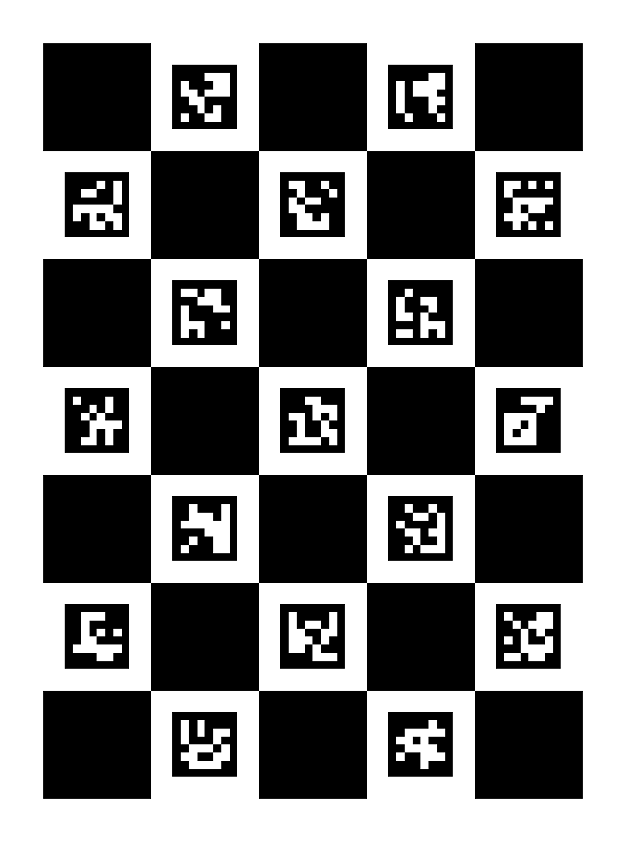
\includegraphics[width=\textwidth]{images/registration/charucoboard.png}
    \caption{Chessboard pattern}
    \label{figure:charucoboard}
  \end{subfigure}
  \hfill
  \begin{subfigure}[b]{0.24 \textwidth}
    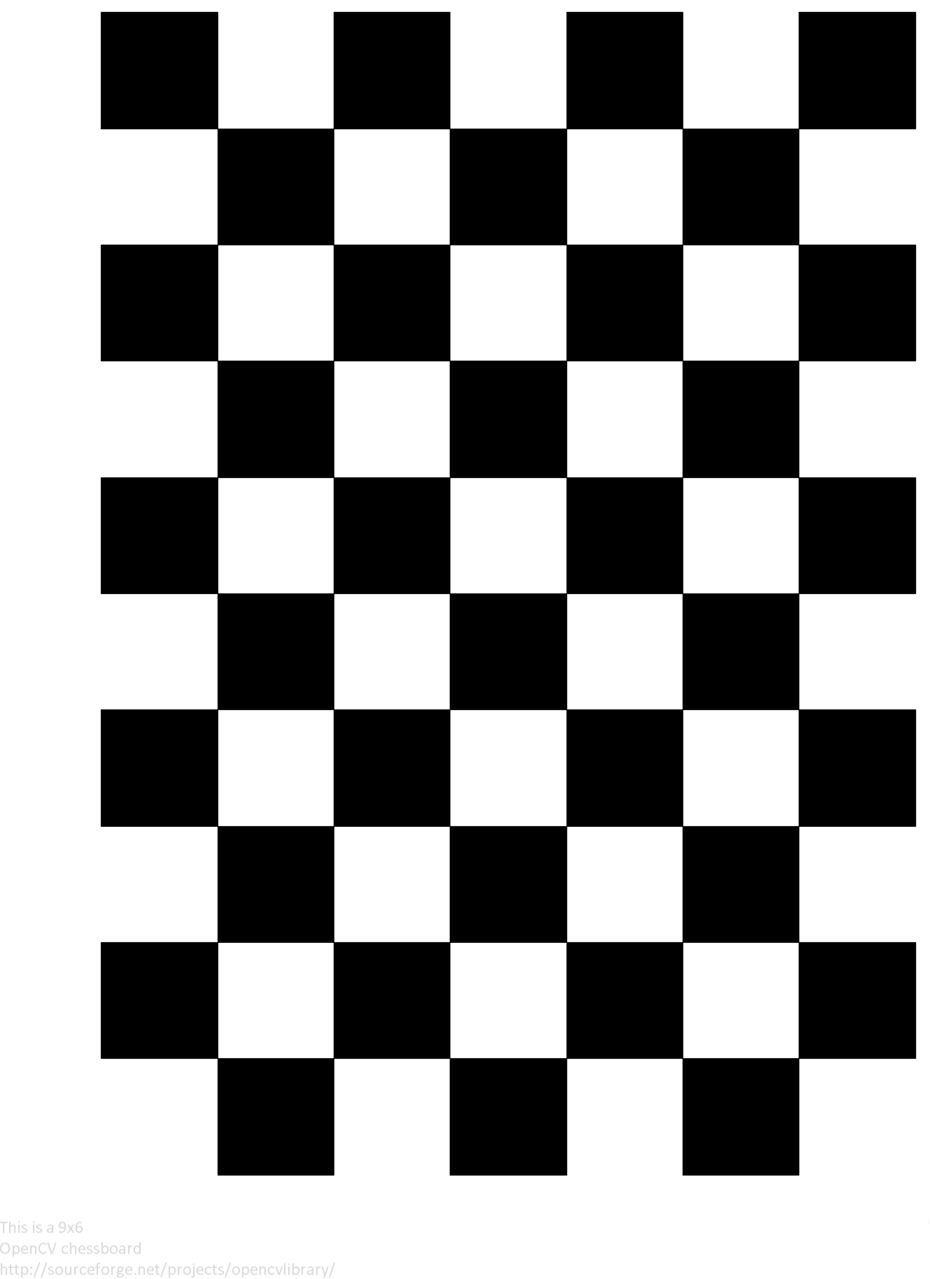
\includegraphics[width=\textwidth]{images/registration/chessboard.jpg}
    \caption{Chessboard pattern}
    \label{figure:chessboard}
  \end{subfigure}
  \hfill
  \begin{subfigure}[b]{0.24\textwidth}
    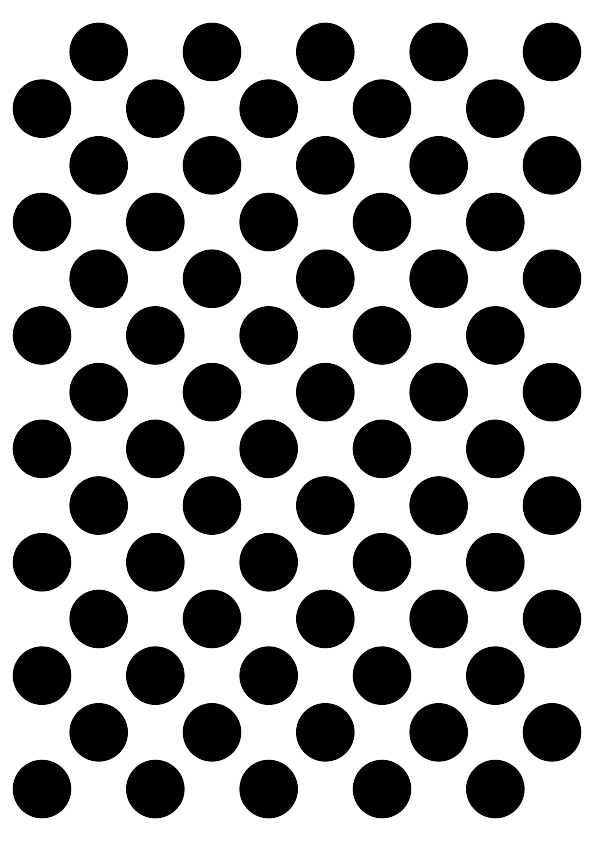
\includegraphics[width=\textwidth]{images/registration/circle_pattern.png}
    \caption{Circle grid pattern}
    \label{figure:circle_pattern}
  \end{subfigure}
  \hfill
  \begin{subfigure}[b]{0.24\textwidth}
    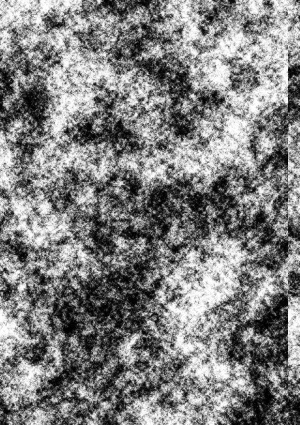
\includegraphics[width=\textwidth]{images/registration/random_pattern.jpg}
    \caption{Random pattern}
    \label{figure:random_pattern}
  \end{subfigure}
  \caption{Easily detectable patterns provided by OpenCV \cite{noauthor_opencv_nodate}}
  \label{figure:pattern}
\end{figure}


\subsubsection{Deep Learning}

Other approaches try to handle this registration problem with Deep Learning. This is the case of \textit{3DRegNet} \cite{pais19} which is a Deep Neural Network for 3D Point Registration. Two tasks are achieved with 3DRegNet:

\begin{enumerate}
    \item Finding 3D points correspondences and classify them into inliers/outliers
    \item Based on the found correspondences, computing the pose of the point clouds to then calculate the transformation matrix.
\end{enumerate}